\chapter{Report on Mathematical Instruction in Italy}

\begin{center}
{\em By}~ ENRICO BOMPIANI
\end{center}

\blfootnote{This address was given at the South Asian Conference on Mathematical Education held on 22-28 February 1956 at the Tata Institute of Fundamental Research, Bombay.}
\setcounter{pageoriginal}{110}
Before\pageoriginale entering on the subject proper of this lecture, namely mathematical instruction in Italy, I think it advisable, or better necessary, to give you a general picture of the educational system in Italy so that, when introduced to details of mathematical instruction, you may understand the different aims of the various kinds of schools, and of their various levels, and see how mathemtical teaching is adapted to them.

Let me point out some difficulties which make themselves immediately apparent when one tries to sketch the educational system in a definite country at a definite moment.

Educational systems differ widely in different countries. They are the final product (at a certain date) of different cultural traditions, of political, geographical and economic conditions : moreover, where culture is really alive, educational systems are continuously changing in order to profit by the most recent scientific acquisitions and to adapt themselves to the varying conditions of the country.

This makes it evident that no system can be really understood without knowing, at least in a general way, its historical background, and that the description of the system at a definite moment completely disregards the fermentation of ideas which will produce the next system. In addition, because of the variety of educational systems in different countries, it is even impossible to translate in a different language the technical denominations adopted in a country. However, since it is necessary to give a translation from Italian into English this can only be an approximate one, and it is\pageoriginale only meant to convey some ideas referring to similar institutions : that is why Italian denominations are also given for exact reference.

This report is divided in two parts. The first gives a general sketch of the present educational system in Italy (different types of schools and their aims; the Ministry of Public Instruction and its role; compulsory education and fees; historical survey of the preceding educational systems). The second part is only devoted to mathematical instruction : programmes, aims, and related information is given for the different types and levels of schools.

\medskip
\begin{center}
{\large\bf Part I}\relax
\bigskip

{\bf The Present Educational System In Italy}
\end{center}
\begin{enumerate}
\item Types of schools at different levels.

\item The Ministry of Public Instruction. Its role.

\item Compulsory education. Fees.

\item Historical survey of the preceding educational system.
\end{enumerate}

\section*{Types of Schools at Different Levels.}

The educational system in Italy is organized in the following categories or levels :
\begin{itemize}
\item[I.] \textsc{scuola elementare o primaria : elementary or primary school.}
\end{itemize}

Children enter this school at the age of 6; it lasts {\em five} {\rm y}ears (from 6 to 11 years of age).
\begin{itemize}
\item[II.] \textsc{scuola secondaria inferiore : lower secondary school.}
\end{itemize}

It lasts {\em three} years (from 11 to 14 years of age) and is subdivided in two branches~:
\begin{itemize}
\item[a.] {\em Scuola Media : middle school} (classical branch) : this is intended to prepare children who will continue their education at higher levels.

\item[b.] {\em Scuola di avviamento}~:\pageoriginale {\em vocational school} : this is a professional-technical training school, which prepares children for practical professional activities : students of this school are not supposed to continue their education at higher levels.  
\end{itemize}

\begin{itemize}
\item[III.] \textsc{scuola tecnica} : \textsc{technical school.} It lasts {\em two} years (from 14 to 16 years of age); this is intended to complete and diversify the professional training (arts and crafts) already received in the vocational school.

\item[IV.] \textsc{scuola secondaria superiore} : \textsc{higher secondary school.}
\end{itemize}

This comprehends two different branches, classical and technical, each represented by various types of schools :
\begin{description}
\item[\rm a.] Classical : 
\begin{itemize}
\item[(1)] {\em Ginnasio-Liceo classico} : {\em Classical Gymnasium and Lyceum}.

It lasts {\em five} years (from 14 to 19 years of age) and prepares for all university departments (Facolta---Faculties). Classical (i.e., Greek-Roman) culture, philosophy and literature are particularly stressed.

\item[(2)] {\em Liceo scientifico} : {\em Scientific Lyceum.} It lasts {\em five} years (from 14 to 19 years of age) and prepares for some university departments (all, except Letters and Philosophy, Law, Medicine) : the accent is put on Science, however against a classical background.

\item[(3)] {\em Liceo artistico} : {\em Lyceum of Art.} It lasts {\em five} years (from 14 to 19 years of age) and prepares for the Department of Architecture. Art is particularly stressed.

\item[(4)] {\em Liceo (Istituto) Magistrale} : {\em Teachers' College.} It lasts {\em four} years (from 14 to 18 years of age) and prepares the future teachers of elementary schools. It may give access to a few University\pageoriginale Departments (Letters, Philosophy, Pedagogy).
\end{itemize}

\item[\rm b.] Technical~: This comprehends various {\em Istituti Tecnici Supriori} : {\em Higher Technical Institutes} with different aims :
\begin{itemize}
\item[(1)] commerce (or trade-school for accountants)

\item[(2)] for surveyors

\item[(3)] industrial

\item[(4)] agriculture
\end{itemize}
They all last {\em five} years (from 14 to 19) and they do not give access to the university.
\end{description}

\begin{itemize}
\item[V.] \textsc{universit\'a : university.} This is divided in various departments (faculties) and leads to a Doctor's degree. In general, it lasts {\em four} years, except for engineering ({\em five} years) and medicine ({\em six} years).

\item[VI.] \textsc{post-unversity institutions.} These are intended to give a further specialization in a definite professional line. They last one or more years; sometimes they are attached to university departments, sometimes they are separate institutions (like the Institute for Advanced Mathematics in Rome, the Institute for High Frequencies in Turin, and many others).
\end{itemize}

The connections between schools at one level and the next (as well as the various university departments) are shown in Table \ref{chap9-tabI}.

\begin{itemize}
\item[2.] \textsc{The Ministry of Public Instruction. Its Role.}
\end{itemize}

The educational system in Italy is governed by a Ministry of Public Instruction : the Minister is a Cabinet member and reports yearly to the Chambers (Parliament and Senate) for the approval of the budget.

The Ministry comprehends seven general directions (or divisions) : for elementary education, secondary technical education, secondary classical education, universities, fine arts, museums and libraries, cultural relations with foreign countries, administration, and is 
\begin{table}[H]
\centering
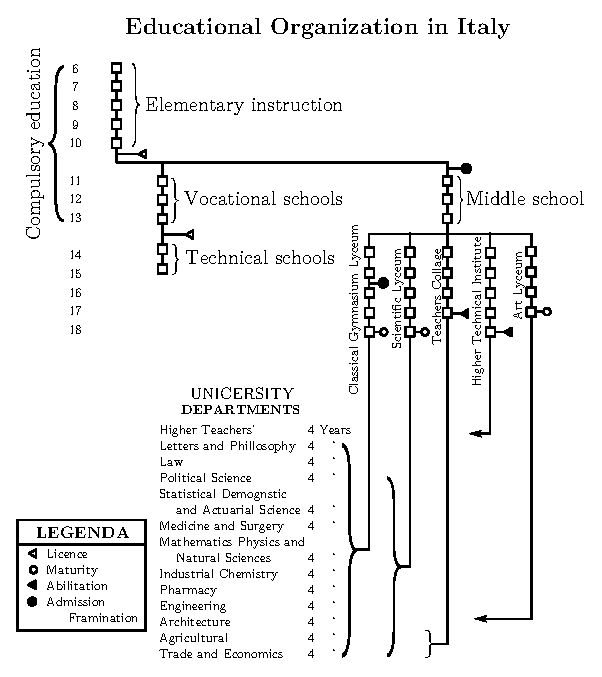
\includegraphics{figure/tab_01.eps}
\caption{}\label{chap9-tabI}
\end{table}

\newpage

\begin{figure}[H]
\centering
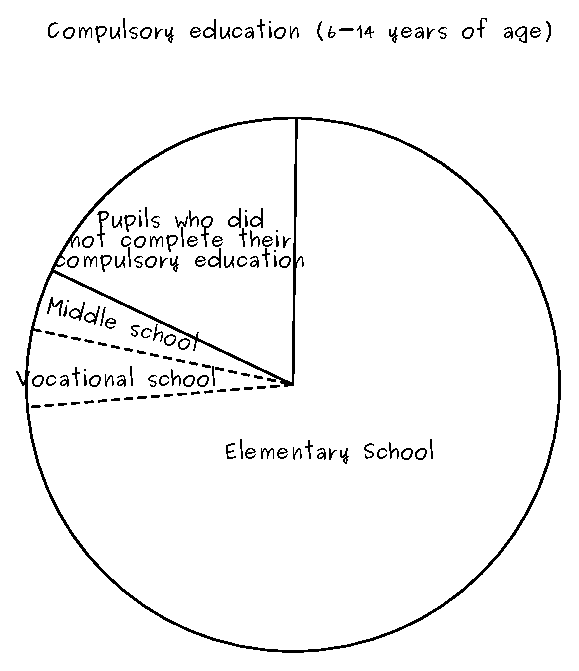
\includegraphics[scale=.85]{figure/fig_38a.eps}
\end{figure}


\setcounter{pageoriginal}{116}
\noindent
assisted\pageoriginale by the Higher Council of Education divided in different sections (elementary, secondary, university) whose members are teachers and professors elected by their colleagues of the same level (and a few appointed by the Minister).

The Ministry has a double function : it acts as an expert establishing the general standard of education at the different levels and as an administrator.

Schools (at various levels) are divided into two types : {\em state} (or government's) schools and {\em private} schools. These are subdivided into {\em legally recognized} schools and those simply {\em authorized.}

Each school is presided over by a Director or President; all schools (except the universities) of a province (regional section of the State) are under the supervision of a (``provveditore'') representative of the Ministry in that province.

For the state schools the full financial burden for the teaching staff is assumed by the Ministry (other services are partly paid for by the province or local authorities).

Both on state and private secondary schools the Ministry exercises a supervision and a control on the didactic and disciplinary aspects using a selected body of ``central inspectors'' (and, for elementary schools, of ``didactic inspectors'' appointed on a national or regional scale).

The Ministry sets down for each type of school not a syllabus or teaching rules, but the amount of knowledge in the different subjects which must be possessed by the pupil at the end of each year, or at the end of 3, 4, 5 years depending on the type of school. This knowledge is ascertained by written and oral examinations which prove the ``maturity'' of the pupil at the end of the period and constitute either a ``licence'' from the type of school or ``admission'' to the next level (if any).

State schools and legally recognized schools award degrees or diplomas (of ``maturity'' or of ``licence''); authorized schools are\pageoriginale completely free in their programme and do not grant degrees or diplomas : they must only satisfy some general requirements.

Another function of the Ministry is the appointment of new teachers and professors. This is done in different ways at different levels.

At the elementary school level the appointment of new teachers takes place on a {\em regional} scale. The representative of the Ministry in a province (provveditore) announces every second year the opening of a competition and appoints the members of a judging Commission (the slate must be approved by the Ministry). The Commission is composed of a President, a university professor or the Director of a secondary high school or a Central Inspector of the Ministry, and of members who are secondary school professors, and of one elementary school teacher. Candidates, who must have at least a diploma from the Teachers' College, must pass a definite set of examinations, designed to ascertain their cultural fitness and their didactic ability.

Competition for ``didactic inspectors'' (in elementary schools) is on a {\em national} (not regional) basis : candidates must be expert teachers with a certain number of years of actual teaching and with a diploma granted by the Higher Teachers Department (Facolt\`a di Magistero; {\em three} university years).

Competitions for the appointment of secondary school teachers (at all levels) are also on a {\em national} basis. The competition (for each discipline) is announced by the Ministry of Public Instruction which also appoints the judging Commission, two thirds of the membership of which consists of university professors and one third of secondary school professors. Candidates must possess a Doctor's degree in the discipline for which they apply and they are rigorously selected through written and oral examinations which ascertain their cultural preparation and their didactic ability. Only those ``habilitated'' can enter on careers in the teaching professions : after three years of actual satisfactory teaching they are appointed full professors.
\begin{figure}[H]
\centering
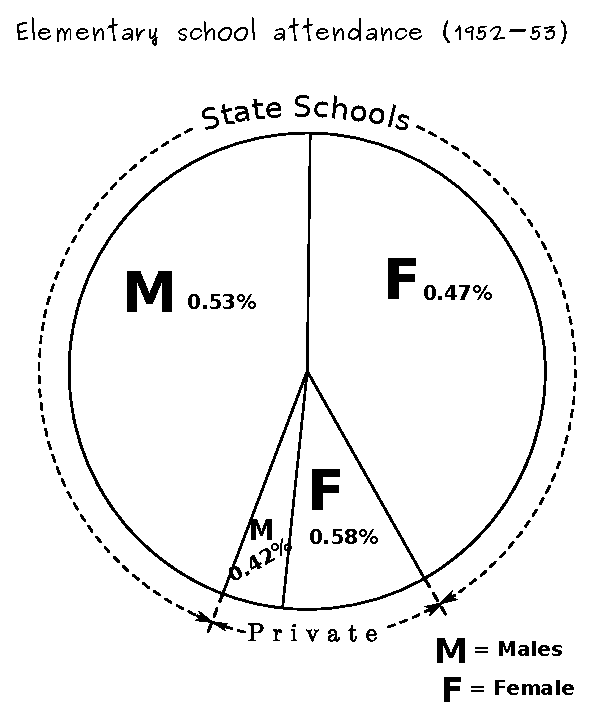
\includegraphics[scale=.9]{figure/fig_38b.eps}
\end{figure}

\eject

~\phantom{a}

\vfill

\begin{figure}[H]
\centering
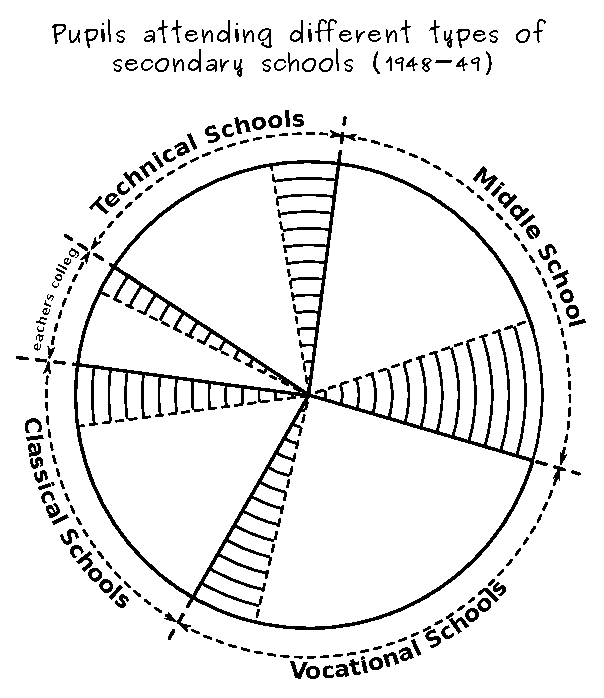
\includegraphics{figure/fig_38c.eps}
\end{figure}

\vfill\eject

\begin{figure}[H]
\centering
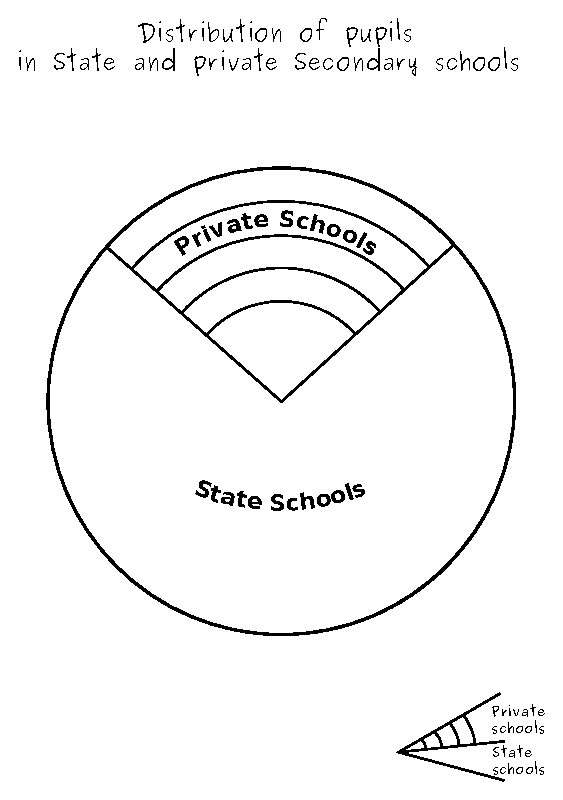
\includegraphics[scale=.9]{figure/fig_38d.eps}
\end{figure}

\begin{figure}[H]
\centering
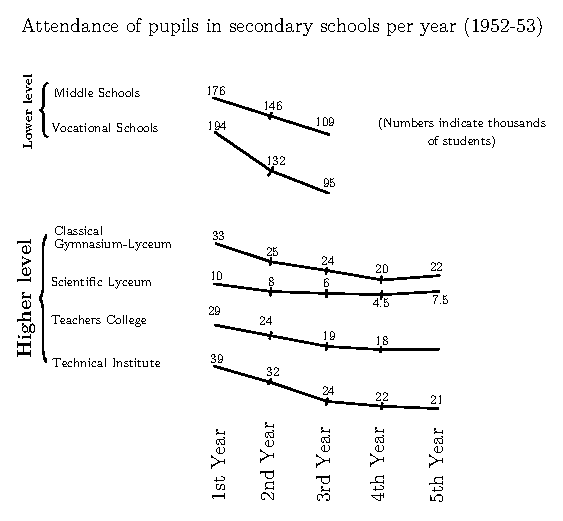
\includegraphics[scale=.9]{figure/fig_38e.eps}
\end{figure}

\setcounter{pageoriginal}{122}
Directors\pageoriginale or Presidents of secondary schools are also selected by the Ministry on the basis of a {\em national} competition among full professors satisfying higher cultural and moral requirements than the average.

The selection of university professor is also the result of a {\em national} competition, of a quite different character.

When the Faculty of a certain department in a university decides to fill a vacant chair (all universities being self-governing bodies) it asks the Ministry to open a competition for that chair. If the application is approved by the Higher Council of Education (an elected body of university professors), the Ministry announces that the competition is open and at the same time invites the staff of the interested department in each Italian university to vote for two full professors in the required subject (for which the chair is vacant) as members of the judging Commission. The five full professors who have received the largest numbers of votes constitute the judging Commission.

Applicants are requested to send to the Commission, through the Ministry, their ``titles'', i.e. their scientific publications, their curriculum vitae, a list of former appointments, and so on.

When the Commission meets, it examines carefully each document of each applicant and then compares the scientific merits of the various applicants : a record of this examination and of the subsequent comparison is later printed in the official bulletin of the Ministry (so that everyone can check the justification of the judgements). The Commission concludes its work by nominating, in order of merit, three winners of the competition; only these can be appointed (even if the number of acceptable choices for a university chair are larger). The Faculty that asked for the competition may appoint any one of the three winners.

The system is so devised as to avoid personal, political or regional interference and to secure the choice of really the best candidate.

Three years after his first appointment, a university professor is subject to a new analysis of his scientific and didactic activities by\pageoriginale a Commission of his senior colleagues; if this analysis ends favourably he is promoted to a full professorship. Not even the Minister can remove him from this position (except in case of moral misdoings, in which case a disciplinary commission is set up to examine his case).

\begin{itemize}
\item[3.] \textsc{Compulsory education. Fees.}
\end{itemize}

Education is compulsory in Italy for all children (boys and girls) from 6 to 14 years of age.

That covers the elementary and the lower secondary level. (Groups I, II in \S 1).

Therefore the elementary state schools and the vocational state schools are absolutely free of charge; the (lower) middle school (which is only a transition school giving access to higher levels) charges an annual fee which amounts practically to the cost of a package of cigarettes.

Actually the higher secondary schools also are practically free of charge : until a few years ago the annual tuition fee for these schools amounted to 70 cents (It. Lire 450); recently it has been raised to \S 3 (It. L. 2000) for the technical high schools and to \S 8 (It. Lire 5000) for the classical high schools. This increase is not intended to cover the government's educational expenses, but to provide financial reserves for fellowships to the most gifted children and for the maintenance of school buildings.

Annual fees for university education oscillate around \S 40 (somewhat higher when operating equipment is required); which is practically only one tenth (or less) of the actual cost of instruction (disregarding all other expenses). It follows that the State is actually supporting by far the largest part of the financial burden of education : this is a necessary consequence of the average economic conditions of Italian families. Nobody, or almost nobody, could afford to pay fees of the order of magnitude exacted in some other countries.

It must also be added that attendance at university lectures is open to anybody. There are no prerequisites laid down, and the instruction\pageoriginale is completely free of charge, provided the attendant does not ask for any certificate or diploma.

\begin{itemize}
\item[4.] \textsc{Historical survey of the preceding educational systems.}
\end{itemize}

I have given in the preceding sections, a sketch of the present educational system in Italy. to understand how it was arrived at, it is necessary to take a glance at its historical background, at its successive developments and changes.

A century ago Italy was still divided into many small states, some of them under foreign domination. Unification of Italy was accomplished only in 1870 with the occupation of Rome (which had been proclaimed the capital town of the new nation already in 1861).

The year 1859 was particularly rich in political and military events : the war of liberation of the northern part of Italy from Austrain domination was actually started.

The fundamental law of public instruction in Italy, known as the ``Casati Act'' goes back to the same year.

Senator Casati, who was already a prominent political leader, was appointed Minister of Education while participating in the war. In the six months he remained in this capacity he fathered an excellent law which remained the corner-stone of public education in Italy.

The importance of the Casati Act is fundamental in many respects : it stressed the concept of freedom of teaching, the universal duty and right to elementary education, common to all social classes of people irrespective of their ability to continue their studies to a higher level, in a really democratic spirit. Elementary education became therefore compulsory and state schools were organized on a five year basis (divided in two periods or cycles) completely gratuitous. The State character of these schools not only removed from the elementary education the influence of particular groups, made them accessible to everybody and erased all\pageoriginale social class distinctions but was largely instrumental in bringing about the spiritual unification of Italy, giving a common pattern of education to all Italian regions.

Not less revolutionary was the Casati Act in the field of secondary education. This was at that time. In Italy as well as in other countries, restricted to a limited number of people, run almost exclusively by religious organizations, and was restricted to the study of the humanities in a classical sense. The Casati Act reduced the old Ginnasio from six to five years and added three years of Liceo (extending the secondary education to 8 years). It continued the study of Latin and Greek, but brought in philosophy (which was formerly confined to the university) and the exact sciences (mathematics, physics, natural sciences). The Ginnasio-Liceo, which is still the best and most homogeneous secondary educational system (and almost unchanged since the Casati Act) gives a solid cultural background and a complete picture of all intellectual activities so as to allow the student who is going to enter the university to make a conscious choice of the particular field in which his natural attitudes will be more suited and fruitful.

The Casati Act also provided a professional education for those who did not intend to continue their studies at the university level, creating the technical schools and institutes with clearly stated professional aims.

Later adjustments (1904) extended the compulsory education period from five to six years (between 6 and 12 years of age) and brought about other minor changes.

The next important step, after the Casati Act, was taken by the philosopher Giovanni Gentile in 1923 (at that time Minister of Education in the Fascist Government). He arrived at his reform---called the Gentile Reform Act---in accordance with his philosophic ideas and his large experience as thinker and educator.

It was the merit of the Gentile Reform to extend the compulsory education to 8 years (from 6 to 14 years of age). To this effect ``integration\pageoriginale classes'' (3 years, which later (1929) developed into the vocational and professional training schools) were added to the 5-years elementary classes (3 years of {\em pre-elementary} or nursery school were also added, before the elementary course, but were not compulsory).

One of the aims of the Gentile reform of secondary education was to reduce the number of State schools, in order to give them a higher standard and to encourage private initiative and competition : however, this aim was largely frustrated both by the pressure of an ever increasing population and the successive totalitarian trend of the Fascist Government.

Another important change introduced by the Gentile Reform Act was the suppression of the old technical school and the creation of a Technical Institute with an openly declared professional character and a Scientific Lyceum, of a cultural character, with emphasis put on Sciences and modern languages.

A logical consequence of the extension (to 8 years) of the compulsory education and a further step in the process of socialization of the secondary school was the creation of the {\em Scuola Meida unica} : the {\em single Middle School} (similar to the {\em ecole unique} in France and the {\em Einheitsschule} in Germany) covering three years of work (Bottai Act, 1940). This single type of middle school prepares the youngsters for the four types of higher level : Ginnasio-Liceo (2 + 3 years), Liceo Scientifico (5 years), Lyceum of Art (5 years), Teachers' College (4 years).

The Middle School together with the Ginnasio-Liceo covers the same ground as the Ginnasio-Liceo of the Casati Act which is the traditional Italian school giving access to the university.

The gradual application of the Bottai Act was hindered by war and political events. The constitutional changes which happened after the war and the renewal of the democratic spirit prompted the necessity of a new reform of the educational system. This reform has been prepared by the Ministry, with the cooperation of\pageoriginale a large number of teachers, professors and experts, in the last years : but is still to be approved by the Parliament.

Programmes, except for minor changes (not affecting mathematics), are still those of the pre-war period. An exception must be made for the elementary school, in which new programmes have been adopted this year with a new subdivision in cycles (2 + 3 years).

 
\medskip
\begin{center}
{\large\bf Part II}\relax
\bigskip

{\bf Mathematical instruction in Italy}
\end{center}
\begin{enumerate}
\item Mathematical instruction at the elementary level.

\item Mathematical instruction in Vocational and Technical Schools (lower secondary level).

\item Mathematical instruction in the Middle school (lower secondary level).

\item Mathematical instruction in the Classical Gymnasium-Lyceum (higher secondary level).

\item Mathematical instruction in other types of Lyceums (higher secondary level).

\item Mathematical instruction in Technical Institutes (higher secondary level).

\item Mathematical trends and their impact on textbooks used at the secondary level.

\item Mathematical instruction at the University level.
\end{enumerate}

\begin{itemize}
\item[1.] \textsc{Mathematical instruction at the elementary level}.
\end{itemize}

As already noted the elementary five-year course is divided in two cycles $(2+3)$.

In the first cycle children begin their acquaintance with integers (from 1 to 20 and then from 21 to 100), with the writing and reading of\pageoriginale integers and the four operations on them (always avoiding remainders in the division).

The Pythagorean table is constructed and memorized.

Of course the teaching of numbers and operations on them is not done in an abstract way : the teacher must use every opportunity to show their necessity, following from very simple (one-operational) problems arising in their games or in practical life.

The intuition of the space is derived from direct observation of the most common objects (desks, chairs, cubes, spheres) and attention is drawn to some plane elementary figures (squares, triangles, circles) possibly showing their relations to solid objects.

In the second cycle the teaching of mathematics, although always connected with the other subjects of the cycle and always drawing its suggestions from practical problems, gradually differentiates itself and acquires a certain amount of autonomy. Operations are extended to integers greater than 100 and to decimal numbers (with no more than three digits). The idea of fraction is given (avoiding operations on them). Particular stress is put on mental operations even approximate. The metric system is also taught avoiding the use of less common units of measure. Children are drilled in recognizing the kind of operation required in one-operational problems : t the end of the cycle they must be able to solve problems involving at most three simple operations (exceptionally four).

In geometry, children must be able to calculate perimeters and areas of simple geometric figures (squares, rectangles, triangles, circles, up to regular polygons); and the volumes of very simple solids.

They are also encouraged to suggest, formulate and solve practical problems drawn from their own experience.

\begin{itemize}
\item[2.] \textsc{Mathematical instruction in Vocational and Technical Schools (lower secondary level).}
\end{itemize}

Access is given to the vocational school by a ``licence'' from the elementary school.

It\pageoriginale is intended to give notions of arithmetic and geometry necessary to practical life, particularly in the branch of activity (arts and crafts) children intend to develop.

The instruction comprehends arithmetic and geometry : to it 9 (weekly) hours are devoted $(4+3+2)$.

The first year comprehends only arithmetic : children are drilled again in oral and written exercises on the four operations so as to insure a full command of them. Powers with integer exponents are then introduced both for integer and decimal numbers. In the arithmetic of integers the concept of prime number is introduced, the factorization of an integer in prime numbers and the research of the g.c.d. and l.c.m. are performed. Fractions and operations on them are also part of the first year programme.

In the second year the rule to extract the square root of a number is given and children are drilled in the use of numerical tables. Letters are introduced to represent numbers; simple equations of the first order with one indeterminate are solved. Non-decimal systems are taught for measure of time and angles.

The second year programme includes also geometry : segments, angles and their measures, perpendicular and parallel lines, polygons (in particular regular polygons and their properties) circumferences and circles, their arcs, chords, angles on the circumference and their measures are part of it. Properties of plane figures with respect to movements and the theory of equivalence are also given.

In the third year the programme of arithmetic comprehends the theory of proportions, interest investments, discount and mixture problems; in geometry proportionality and similitude (Thales theorem), and also measure problems, measure of areas and volumes of parallelopipeds, pyramids, cones, spheres, are developed.

Teaching of mathematics in vocational schools is mainly on a practical intuitive basis; it is however advised not to discard completely the deductive method when experiment can only be used for checking results.

The\pageoriginale technical schools, to which access is given by a licence examination from the vocational school, are largely differentiated in accordance with the various activities they are intended to prepare the student for (mechanics, engineers, electricians, radio experts, traders, agrarians, and so on). Also, the time devoted to mathematics differs from type to type, according to the special needs. The principal aim is to give the students a real command in the use of all notions already apprehended, in particular the units of measures, to be used in allied subjects (mechanics, physics, electrotechnics); large use is made of numerical tables, logarithms, slide rules, cartesian co-ordinates, graphs, circular functions, trigonometry of the right-angles triangle.

\begin{itemize}
\item[3.] \textsc{Mathematical instruction in the Middle School (lower secondary level).}
\end{itemize}

The (single) Middle School, as was previously said, is intended for those children who will continue their studies at a higher (university) level. Hence, admission is restricted by higher requirements.

Having completed their elementary classes, applicants must pass an admission examination : the judging Commission is composed of secondary school professors assisted by an elementary teacher. The examination as far as mathematics is concerned, consists of a written test (solution of a problem implying three operations at most) and of an oral test in which the candidate must show his fitness for more advanced studies.

The teaching of mathematics in the Middle School has two aims : (a) to increase the amount of mathematical knowledge already acquired in the Elementary School; (b) to prepare the youngsters for the study of rational mathematics and abstract thinking.

To accomplish these, although intuitive-empirical help must not be banned, the student is required to be precise in his concepts and their verbal expression. Teachers are asked to couple their teaching with some general mental operations, like ordering, partitioning, assembling, proportioning, equating.

The\pageoriginale time devoted to mathematics is 9 (weekly) hours $(3+3+3)$.

In the first year, operations on integers are reconsidered in order to put in evidence their formal properties (reflexive, associative, commutative, distributive laws) and the reasons for the practical rules already learned in the elementary school. The use of parentheses is emphasized. Then new concepts are introduced : the power (to an integer exponent) of a number, the prime numbers, the factorization of an integer in prime numbers, the research of common divisors and multiples, in particular of g.c.d. and of 1.c.m. of two or more integers (also by the Euclidean process of successive divisions), the fractions and the operations on them.

Geometry in the first year of the Middle School is mainly intuitive, in order to introduce the knowledge of geometrical figures to be studied rationally on the next level : segments, lines, angles, perpendicularity and parallelism of lines, triangles, parallelograms and so on.

In the second year, after completing the operations on fractions, decimal numbers are considered (limited or periodical and their generating fractions); the rule to extract the square root and the theory of proportions also belong to this year. In geometry, properties of elementary geometric figures (including Pythagoras theorem, the rectification and quadrature of the circle) are given mainly in an intuitive way, but not discarding simple deductions as an inducement to mathematical thinking.

In the third year, relative numbers are introduced and operations on them. Here also begins algebra, with the use of letters, introduction of monomials (and their similarity), of polynomials, of the three operations (except division) on them, factorization in simple cases and remarkable identities. In geometry, circumference and circle and their measures are considered again not simply giving the rules for their calculation but indicating the geometric procedures which lead to them (inscribed and circumscribed regular polygons). A large number of applications of the elements of algebra to\pageoriginale geometric problems (particularly on the Pythagoras theorem) is suggested.

In solid geometry, relative positions of lines, of lines and planes, are also part of the syllabus.

Historical information about outstanding mathematicians (like Euclid, Pythagoras, Thales) is advised (but not compulsory).
\begin{itemize}
\item[4.] \textsc{Mathematical instruction in the Classical Gymnasium-Lyceum (higher secondary level).}
\end{itemize}

Students enter the higher secondary level (Lyceums and Technical Institutes) after having passed their licence examinations from the Middle Schools.

I shall give in this section a sketch of mathematical instruction in the traditional Italian classical high-school : the Gymnasium-Lyceum. In the next section I shall compare the other types of Lyceums with this one.

Teaching of mathematics in the Classical Gymnasium-Lyceum has as its main purpose the developing and disciplining of the natural mental gifts of the student. It is not the material covered which is of paramount importance, but the method of acquisition of the results. Mathematics is not considered as a goal in itself, but a powerful instrument for the refinement of thinking in general : it is inductive to creative thinking, and also to clear cut ideas, to their exact verbal formulation; it establishes the habit of controlling one's own process of thinking and of intellectual honesty.

Besides that, mathematics and particularly geometry is an integral part of the Greek (classical, in a Western sense) culture which would be badly mutilated and misrepresented if mathematics in the rational form should not appear in the syllabus of a Classical Lyceum.

As to the method of teaching : it must not be a purely logical exercise based on a certain set of postulates, but these must spring out of commonsense experiment and intuition retracing their historical\pageoriginale and psychological origin : the raw materials already assimilated in the lower level are subjected to a logical re-examination to find out the first principles (postulates) from which the same conclusions can be drawn.

The Gymnasium-Lyceum consists of 2 years of Gymnasium (which one enters with the licence of the Middle School) and 3 of Lyceum.

In the {\em Gymnasium} 4 (weekly) hours $(2+2)$ are devoted to mathematics. Rational positive and negative numbers are introduced and operations on them, including powers with a relative integer exponent. Algebra includes polynomials and operations on them, basic products, factorization; algebraic fractions and operations on them, and the solution of equations of the first degree. Geometry starts with the usual elements (lines, half-lines, segments; planes, half-planes, triangles and polygons) and gives the criteria of equality of triangles, theorems on perpendicular and parallel lines, the sum of internal and external angles of a polygon, the triangular inequalities, properties of parallelograms in general and in particular cases; theorems on relative positions of lines and circles or of circles in a plane, angular properties of a circle; regular polygons and their properties, and some fundamental graphical problems. The theory of equivalence is developed for polygons up to and including Pythagoras theorem.

In the {\em first class of the Lyceum} (3 hours weekly), algebra is continued with the solution of systems (of no more than three) linear equations. The concept of real number is then introduced and operations on real numbers, including powers with integer or rational exponents (calculus of radicals). Then quadratic equations are discussed and solved, and systems of non-linear equations leading to resolution of quadratic equations are also solved.

In geometry the theory of proportions of geometric magnitudes is given; the similitude of triangles and polygons, the theory of measure and the area of polygons, are also developed rigorously.

In\pageoriginale the {\em second class of the Lyceum} (2 hours weekly) the syllabus comprehends : the theory of arithmetic and geometric progressions, of exponential equations and logarithms, with numerous exercises and applications requiring the use of logarithmic tables.

In geometry : rectification of the circumference and quadrature of the circle are rigorously carried out. Solid geometry begins with notions of lines and planes and their relative positions; orthogonality and parallelism, dihedra, trihedra and angoloids, polyhedra (in particular prisms and pyramids), cylinder, cone and sphere are studied.

In the {\em third class of the Lyceum} (2 hours weekly) geometry and trigonometry (with graphs of trigonometric functions, addition formulas and so on) are developed up to and including the resolution of triangles (Carnot theorem, Sines theorem and their applications).

In geometry the theory of equivalence of polyhedra and the rules to determine areas and volumes of other solids are studied.

In all classes numerous applications are made of algebra to geometry.

As to the teaching methods, or better lines of development and proofs, the teacher is absolutely free to choose those he prefers. For instance, real numbers are introduced either using contiguous classes and Dedekind sections or the decimal representation of numbers. Equivalence of polygons can be introduced either using decomposition in equal parts, or using the postulates for equi-extension of two figures (Severi).

Equivalence of polyhedra is developed either using the ``Cavalieri principle'' (equivalence of parallel plane sections) or, for prisms, the decomposition in equal parts, or finally, for pyramids, the method of ``scaloids''.

The theory of proportionality of geometric magnitudes is either reduced to numerical proportions, using their measures, or is given using the original Euclidean method (comparison of equi-multiples). And so on.

\begin{itemize}
\item[5.] \textsc{Mathematical\pageoriginale instruction in other types of Lyceums (higher secondary level).}
\end{itemize}

I shall report in this section on mathematical instruction in the other types of schools of classical character (Scientific Lyceum, Lyceum of Art, Teachers' College) referring to the Classical Lyceum and putting in evidence their differences with it. The character of the teaching is always the same (i.e. rational, and conceived as part of a general cultural frame), but more or less emphasis is put on mathematics with respect to other subjects.

In the five years of the Scientific Lyceum mathematics plays a major role. The time devoted to it is considerably larger than in the Classical Lyceum ($5+4+3+3+3=18$ weekly hours as against 13 in the last type) and so is the syllabus. The following subjects are to be added.
\begin{enumerate}
\item Elements of plane analytic geometry : Cartesian co-ordinates, graphical representation of functions of one variable (line, circumference, parabola with its symmetry axis parallel to one of the coordinate axes, hyperbola with the asymptotes parallel to the axes; logarithmic curve and graphs of trigonometric functions).

\item Elements of infinitesimal analysis : limits, derivatives of elementary functions (with their geometric and physical interpretation); problems on maxima and minima; definite and indefinite integrals.

\item Combinatory calculus : dispositions, permutations, combinations, Newton's formula for the expansion of the power of a binomial.
\end{enumerate}

Particular stress is put on the discussion of the solutions of a quadratic equation whose coefficients depend on a parameter (interval of the variability of the solutions, their reality, in correspondence with the interval of variability of the parameter); geometrical problems relating to this situation are largely discussed. The comparison of the solutions of a quadratic equation with a real number is made by different methods (direct comparison; Cartesian\pageoriginale rule and its extension; method of the fixed parabola; Tartinville's method).

As for the distribution of the subjects in different years, the first year in the Scientific Lyceum covers the same programme as the first two years of the Classical Lyceum (Gymnasium); analytic geometry starts in the second year and the elements of analysis in the fourth year.

In the {\em Art Lyceum}, the teaching of mathematics is coupled with that of physics and comprehends in all 17 hours $(4+4+4+5)$. The syllabus is practically the same as in the Scientific Lyceum. It is to be said that owing to the particular aims of this kind of Lyceum, a lot of descriptive geometry (method of orthogonal projections, perspective and their applications) is given in the courses of ``geometrical design'' and ``perspective'' covering all together 15 hours weekly $(4+3+4+4)$.

In the {\em Lyceum for Teachers} (or Teachers' College) the teaching of mathematics has a twofold purpose also : to promote the scientific culture of the pupils, and to give them the necessary professional fitness.

The teaching of mathematics takes up 12 hours weekly $(5+3+2+2)$.

Algebra goes as far as the resolution of systems of linear equations and the theory of quadratic radicals.

Geometry covers the same ground as in the Classical Lyceum except for the fact that some subjects (real numbers, rectification and quadrature of the circle) are not developed in a fully rational manner.

On the other hand (because of the professional need for it) rational arithmetic is part of the syllabus.

\begin{itemize}
\item[6.] \textsc{Mathematical instruction in Technical Institutes (higher secondary level).}
\end{itemize}

Technical Institutes, which in some cases do give access to a limited number of university departments, supply a highly qualified and\pageoriginale specialized technical preparation for various professional activities and are therefore largely differentiated.

The Technical Institutes prepare for the following main professional activities : Commercialists (administrative personnel); Land Surveyors; Agrarians; Nautical personnel (sea-captains, naval carpenters, engineers); Industrialists. These main categories (and particularly the last one) are sub-divided in numerous sub-sets (according to the various specializations) : the syllabus is highly differentiated (particularly in mathematics) to achieve the best preparation in the special field chosen by the student.

It would take too long to give a detailed account of mathematical subjects taught for the various categories of specialization.

It may suffice to say that mathematical instruction has a professional, not a cultural, aim. Financial and actuarial mathematics and calculus of probability have a paramount interest for commercial activities; sea-captains need spherical trigonometry; contractors must know not only accounting but also some of the mathematics used in engineering problems; fine technicians must know how to measure the length of curves on a curved surface; electricians, radio-technicians, opticians, designers need a different mathematical knowledge.

The number of hours devoted to mathematics is different in the various specializations and is generally confined to the first three of four years of the Technical Institute.

\begin{itemize}
\item[7.] \textsc{Mathematical trends and their impact on textbooks used at the secondary level.}
\end{itemize}

Having given you a picture of mathematical instruction at the secondary level, and before passing to the analogous subject at the university level, it seems pertinent to say something about the textbooks used; particularly to put in evidence the impact on them of the modern criticism on the foundations of geometry.

It will appear that outstanding mathematicians in Italy have always had a deep interest in secondary teaching and taken an active\pageoriginale part in writing textbooks, thus ensuring a high scientific level to secondary mathematical instruction (needless to say, there remain a large number of textbooks not satisfying this requirement).

At the beginning of the nineteenth century, mathematical textbooks were mere translations of foreign (particularly French) textbooks : Clairaut's {\em Elements de G\'eom\'etrie}, Legendre's {\em El\'ements de Geometrie}, both remarkably different from Euclid's original Elements, were widely spread in Italian translations so were the {\em Le\c{c}ons nouvelles de G\'eometrie \'elementaire} by Amiot (and Baltrer's {\em Elements of Mathematics}, translated by Cremona).

It was the merit of three outstanding mathematicians, Cremona, Betti and Brioschi to re-establish the teaching of geometry on the original Euclidean text (of which Betti and Brioschi gave an Italian translation in 1867). Having in mind pure scientific research at a higher level, Brioschi and Cremona stated that ``our Gymnasiums and Lyceums must supply a highly elevated culture'' and that their main purpose was ``to teach the youngsters how to reason correctly, how to prove, how to make logical deductions; therefore shortcuts and books which mix together geometry, arithmetic and algebra are no good; Euclid is the real text which serves the stated purposes.''

The same fundamental idea, that mathematics must be rigorous or it is not mathematics, was fostered by the analysis of the foundations of mathematics made by Dini, Veronese and Peano. This atmosphere of rigour created a peculiar character, and a permanent interest of university professors in the redaction of Italian textbooks at secondary level.

It immediately bore fruit : after the translation of Euclid by Betti and Brioschi, original textbooks, following Euclid's spirit but with a certain amount of autonomy and with new organizing criteria, were produced by Sannia, D'Ovidio, De Paolis and many others.

Of\pageoriginale paramount importance in moulding the secondary teaching were ``{\em The principles of geometry logically expounded}'' by Peano (1889) and the ``{\em Foundations of Geometry}'' (1891) and the ``{\em Elements of Geometry}'' (1897) by Veronese. In these books, the purely abstract axiomatic-deductive method (completely severed from all physical suggestions) is strongly stressed. Veronese starts with the point (not with the space) and completely rejects the use of movements (as sometimes used in Euclid) assuming the equality of segments (or congruence of pairs of points) as a primitive notion, with no reference to its physical meaning. The same trend is followed in the analysis of the foundations of geometry by Fano, Pieri and Padoa.

This trend reached the peak of perfection in Hilbert's ``{\em Grundlagen der Geometrie}'' (1898).

It is the merit of F. Enriques, a mathematician combined with a philosopher and a historian, to bring, using the collaboration of U. Amaldi, the results of this critical movement to the secondary school level with their numerous textbooks.

Against the excesses of purely abstract axiomatic teaching at the secondary level, was the reaction of Peano (who insisted that giving a minimal set of postulates or proving every theorem was not necessary; but that only exact statements should be given) and the two philosophers and mathematicians G. Vailati and E. Rignano.

Enriques went a step farther : his philosophical mind was not satisfied with the purely formal perfection reached in geometry; therefore he started an investigation of the psychological ground of our assumptions (see his ``Problems of Science''). On this ground he devoted a tremendous amount of work to didactical problems and to showing the impact of advanced theories on secondary mathematical instruction (following the example of F. Klein's ``{\em Elementar Mathematik vom hoheren Standpunkte aus}''). He also developed a mathematical society (Mathesis) and founded a periodical concerned with these problems.

A\pageoriginale larger appeal to intuition was made in the numerous textbooks of F. Severi : postulates are derived from everyday experience. He re-introduced the movement as a method of proof, however giving it a firm axiomatic foundation. He also gave many subjects (theory of parallels, of equivalence, proportionality of geometric magnitudes) a new and original treatment.

It is impossible to give here a similar analysis of textbooks in arithmetic and algebra; suffice it to say that also in these fields the interest of university professors in secondary teaching has always produced excellent textbooks (Pincherle, Vivanti, Gazzaniga, Bortolotti, Tonelli, Cipolla, Nicoletti, Sansone).

Resulting from the same interest given by university professors to secondary teaching, are the volumes edited by F. Enriques on questions concerning elementary mathematics and the excellent encyclopaedia of elementary mathematics edited by L. Berzolari : practically all Italian university professors took part in these enterprises.

As a further proof of the continuous interest of university professors in secondary mathematical instruction, let me remind you that it was at the fourth International Congress of Mathematicians in Rome (1908) that the International Commission on Mathematical Instruction was born : the resolution, later adopted by the Congress, which was its act of birth, was put on the floor by my unforgettable teacher G. Castelnuovo; among the first members of the Commission were G. Vailati, G. Castelnuovo, F. Enriques, G. Scorza.

\begin{itemize}
\item[8.] \textsc{Mathematical instruction at the university level.}
\end{itemize}

The bulk of mathematical instruction at the university level is given in the Department (Facolt\`a) of Physics, Mathematics and Natural Sciences. Other mathematical courses are given in the Departments of Political Sciences, of Statistical, Demographic and Actuarial Sciences, of Economics, and so on. It would take too long and be of little interest to report on all these special courses; but it would also be, in a certain sense, useless because, since the Gentile Reform Act, a student is free to take some courses also in departments\pageoriginale other than those of his specialization (e.g. a student of philosophy can take courses in mathematics or vice versa; and this actually happens).

Let us confine ourselves therefore to the main mathematical courses. These are divided in two 2-year terms : the first biennium and the second biennium.

Students entering the first biennium must have a licence (after a maturity examination) either from the classical or the scientific Lyceum.

Mathematical courses in the first biennium are compulsory for students of engineering, of mathematics and of physics (chemists can take the same courses or alternatively follow analogous courses specially devised for them). The courses are labelled as follows :
\begin{enumerate}
\item Mathematical analysis (finite and infinitesimal); a two-year course (3 hours of theoretical lectures, 3 hours of exercises and applications, weekly).

\item Analytic, projective and descriptive geometry; a two-year course (with the same schedule as above).

\item Rational mechanics with graphical statics; this is a one-year course, given in the second year of the biennium (4 hours of theoretical lectures, 3 hours of applications).
\end{enumerate}

I have purposely used the word ``labelled'' because the label does not actually indicate the composition of the course or its extension, nor the way it is developed. This is all the more true because courses with the same label differ widely in character from university to university. There is no syllabus defining a course : a skeleton indication is supplied by tradition, but the professor is absolutely free to cover more or less ground and to develop the subject the way he likes. This freedom of teaching finds its expression in the mimeographed (or printed) notes that practically every professor prepares for his students : only these notes define the course; they reflect the personality of the individual professor.

As\pageoriginale an instance, a course in mathematical analysis contains the usual notions of algebra (including the theory of equations), of limits, of series of functions, differential and integral calculus (with multiple integrals), series developments, Laplace transforms and inverse transforms, theory of differential equations and systems of them, partial differential equations : but it may contain other subjects and in any case, different emphasis is put on these various subjects by different professors. Common to all of them however, is the emphasis on mathematical rigour.

The same is true of the geometry course : it certainly includes plane and solid analytic geometry, projective and descriptive geometry; but projective geometry may be treated either synthetically or analytically.

The group idea is in some cases assumed as the fundamental idea of the treatment of the subject.

Besides that, this course contains many topics (singular points of curves or surfaces, linear systems of algebraic curves, Plucker formulas for an algebraic curve, differential study of curves and surfaces in the ordinary space up to and including the fundamental quadratic differential forms) which may be characterized as introductory to algebraic and differential geometry.

As mentioned above, these courses are compulsory for different groups of students (who, besides these, have other compulsory courses which differ for different groups). This fact ensures that mathematical instruction for engineers is on a pretty high level : a few topics however are added to the general syllabus, for prospective professional mathematicians.

Written and oral examinations are required at the end of each course.

After the first biennium, different groups have different curricula and we will follow only the students of mathematics. These continue their studies for a second biennium aiming at a Doctor's degree either in mathematical sciences, or in mathematics and physics. Generally\pageoriginale speaking, the first type of doctorate is chosen by those who want to continue in research work and scientific activities; the second type is devised for those who want to become professors of mathematics and physics at the secondary school level (at this level, since the Gentile Reform Act, the teaching of mathematics and physics is entrusted to the same teacher).

The curricula followed to attain either of the two types of doctorate are pretty similar : in the second type, mathematics and physics are equally balanced and attention is paid to teaching problems.

The curriculum of the second biennium for the Doctor's degree in mathematical sciences comprehends three compulsory subjects : higher analysis, higher geometry and mathematical physics, and three more courses (so-called complementary) which can be chosen by the student among the following : astronomy, numerical and graphical methods of calculation, theoretical physics, advanced physics, algebraic geometry, differential geometry, higher mathematics, theory of functions, complementary mathematics, advanced mechanics, theory of numbers, geodesy, topology, probability, calculus, actuarial mathematics, history of mathematics.

The curriculum of the second biennium for the Doctor's degree in mathematics and physics comprehends four compulsory subjects : advanced physics, higher analysis, theoretical physics, complementary mathematics, and three courses chosen among those already mentioned and many others relating to physics (electro-technique, technical physics, geophysics, mineralogy, spectroscopy, statistical mechanics, electromagnetic waves).

Each course consists of three hours weekly of lectures on theory (with exercises or laboratory work if required) : examinations at the end of the course are required.

Courses at his level are of monographic or research character and their content varies from year to year; the teacher is completely free and is alone responsible for the choice of the topics, which are generally related to his own scientific work at the time. Labels are, on\pageoriginale purpose, very general and indeterminate. Higher analysis may mean a course on calculus of variations, or on operational calculus, or on partial differential equations and so on; mathematical physics may mean optics or elasticity or electromagnetism and so on; differential geometry may mean Riemannian geometry, theory of connections, theory of groups and many other subjects.

As a rule, no textbook is adopted (which would limit the originality of the course); sometimes mimeographed notes are prepared by the professor but generally students are required to take their own notes.

When the student has completed his examinations he must prepare a written dissertation on a subject he chooses freely (generally under the guidance of one of his professors) : the dissertation must show his ability to do scientific research (this requires, in many cases, an additional year).

When the dissertation is approved, the student applies for admission to the final doctorate examinations : these consist of a written and oral ``cultural examination'' (a kind of general survey of the candidate's knowledge in mathematics or in mathematics and physics); of an oral exposition of the written thesis and of three oral theses before a full commission of eleven professors.

If everything goes smoothly he is proclaimed a Doctor; that is the end of his studies and there begins the competition for a teaching post or the fulfilment of scientific ambitions.

\bigskip
\medskip

{\fontsize{9pt}{11pt}\selectfont
University of Rome
}\relax

